\chapter{Realisierung}

Im folgenden Abschnitt soll auf die Implementierung des \textit{Smart Warehouse} Szenarios eingegangen werden. Insbesondere werden Probleme während der Umsetzung der beiden Objektdetektoren \textit{SSD} und \textit{YOLO} betrachtet, die Realisierung der Dashboard-Webapplikation und des Zählalgorithmus zur Durchführung der Inventur aufgezeigt und letztendlich Herausforderungen im Rahmen der Drohnen Anbindung besprochen.

\section{Umsetzung der Objektdetektoren}

\subsection*{SSD}

Für den \textit{SSD} wurde wie bereits erläutert nicht die ursprüngliche Referenzimplementierung im \textit{Caffe} Framework verwendet, sondern eine Custom-Implementierung in \textit{PyTorch}. Diese realisiert die \textit{SSD300} Variante. Neben kleineren Änderungen in der Codebasis zur Erreichung von Kompatibilität mit aktuellen Bibliotheksversionen und weiteren Anpassungen zur Integration eines eigenen Datenbestandes, wurden vor allem zwei größere Erweiterungen durchgeführt. Da der erstellte Datenbestand nur 1088 gelabelte Daten enthält, wurde zusätzlich zur Custom-Implementierung ein fünffaches Kreuzvalidierungsverfahren realisiert. Es dient dazu ein höheres Abstraktionsvermögen des Modells auf dem geringen Datenbestand zu erreichen. Auch unterstützte die Referenzimplementierung keine Validierung durch zuvor ungesehene Daten. Die Modellklassen des Datenbestandes un die Validierungsskripte wurden dahingehend angepasst.

Die Referenzimplementierung erstellt sich des Weiteren einige Hilfsdateien, in der die Pfade zu Bildern und weitere Datenstrukturen für Trainingszwecke abgespeichert werden. Ohne diese ist kein Training möglich, das Trainingsskript fordert demnach Zugriff auf den Sekundärspeicher. 

Um ein lokales Training auf der \textit{NVIDIA GTX 1080} GPU zu ermöglichen, wurde zudem \textit{CUDA} Version 10.1 verwendet. Trainiert wurde mit folgenden Hyperparametern:
\begin{itemize}
	\item Batch Größe: 16
	\item Lernrate: $1.0\cdot e^{-3}$
	\item Momentum: 0.9
	\item Kreuzvalidierungen: 5
	\item Epochen: 120
	\item Gradientenverfahren: Stochastic Gradient Descent
	\item Kostenfunktion: Smooth L1
\end{itemize}

Das Basisnetzwerk des \textit{SSDs} besteht aus einem auf \textit{ImageNet} vortrainierten \textit{VGG16}. Die restlichen \textit{Convolutional Layer} sind \textit{Xavier} initialisiert. 

Die Hyperparameter sind nahezu gleich zu denen in der ursprünglichen wissenschaftlichen Veröffentlichung. Wesentlich die Batch Größe im \textit{Mini-Batch} Verfahren wurde für größere Stabilität von 32 auf 16 heruntergesetzt. Auch in der Evaluierung wurde die Batch Größe von 64 auf 48 herunter gesetzt, da die Eingangsdaten eine weitaus höhere Auflösung als die ursprünglich im \textit{PascalVOC} verwendeten Daten haben. Andernfalls wird Gefahr gelaufen einen Speicherüberlauf zu erzielen. 

\subsection*{YOLO}

Bei \textit{YOLO} kommt das \textit{Darknet} Framework zum Einsatz, eine Implementierung in C. Vor der initialen Kompilierung müssen einige Konfigurationsschritte unternommen werden, weil auch der Betrieb auf einer normalen CPU oder einer GPU mit Tensor Kernen möglich ist. Für das Training kommt eine \textit{NVIDIA RTX 2060 SUPER} GPU zum Einsatz, deren enthaltenen Tensor Kerne mitbenutzt werden. Die benötigten Hyperparameter wurden dabei wie folgt gesetzt:

\begin{itemize}
	\item Batch Größe: 64
	\item Subdivisions: 16
	\item Lernrate: $1.0\cdot e^{-3}$
	\item Momentum: 0.9
	\item Maximale Anzahl Batches: 18000
\end{itemize}

Im Unterschied zum \textit{SSD} kann \textit{YOLO} die in den GPU Speicher zu ladende Datenmenge eines Batches durch sogenannte \textit{Subdivisions} festgelegt. Hierbei werden nur noch $Batch Größe \mathbin{/} Subdivisions$ Bilder gleichzeitig in die GPU geladen werden, um einen Speicherüberlauf zu vermeiden. Bei \textit{SSD} muss immer die gesamte Batch Größe in den GPU Speicher geladen werden oder gegebenenfalls die Batch Größe wie oben reduziert werden, was hinsichtlich des Gradientenverfahren womöglich nicht gewünscht sein kann.

Die Lernrate sowie das Momentum bleiben wie in der Dokumentation empfohlen unverändert zu den Referenzwerten. Im Gegensatz zu \textit{SSD} wird kein Maximum für die Anzahl an Epochen, sondern ein Maximalwert für die zu durchlaufenen Batches gesetzt. Dieser Wert wird abhängig von der Menge an gelabelten Klassen gesetzt und kann als Empfehlung aus der Dokumentation entnommen werden. 

\section{Dashboard Entwicklung}

Der Server wurde mit dem \textit{Flask} Framework in Python implementiert und läuft auf dem \textit{Web Server Gateway Interface} (WSGI) server \textit{Waitress}. Er führt den Inferenzalgorithmus des \textit{SSDs} bzw. des \textit{YOLO} Objektdetektors für jeden Frame des empfangenen Videostreams der Drohne aus und streamt die inferierten Bilder mit den Bounding Boxen an jeden Client. Der Client wurde mit dem \textit{Bootstrap} Framework designed (siehe Abbildung \ref{webapp}).

\begin{figure}[ht]
	\begin{center}
		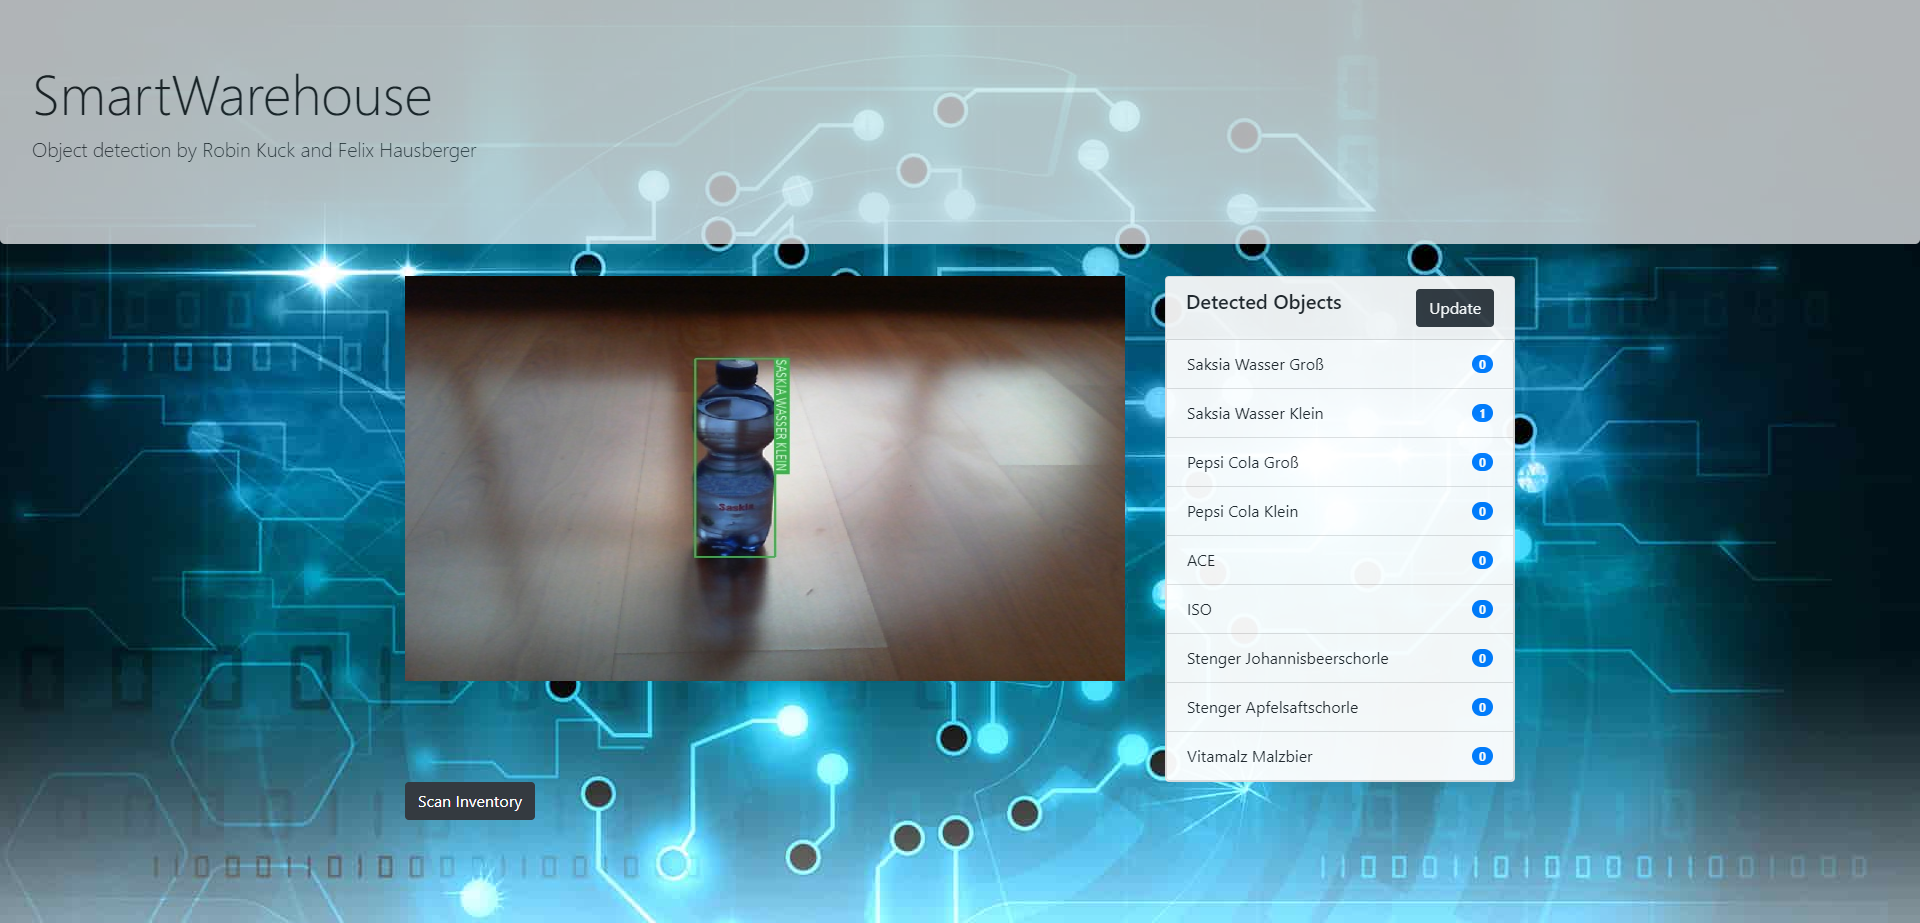
\includegraphics[width=15cm]{Bilder/webapp.jpeg} 
		\caption[Webapp SmartWarehouse]{Webapp SmartWarehouse}
		\label{webapp}
	\end{center}
\end{figure}

Auf Anfrage eines Client kann dieser die aktuell gezählten Objekte vom Server abfragen. Der Zählalgorithmus wird im folgenden Unterkapitel erklärt. 

\section{Zählalgorithmus}

\lstinputlisting[
label={code:formfield},
caption={Zählalgorithmus zum Zählen der detektierten Objekte},
captionpos=b,
basicstyle=\ttfamily\scriptsize,   
firstline=1,              
lastline=11                 
]{Quellcode/algorithmus.txt}

Der obige Algorithmus wird momentan dazu verwendet, um für das Industrieszenario einer Inventur einzelne detektierte Objekte zu zählen. Das Problem, dass der Algorithmus zu lösen versucht, enthält allerdings eine weitere Komplexitätsstufe. Dasselbe Objekt kann im Laufe der Inventur erneut auftreten und dessen relative Position im Bild ist ebenso variabel. In diesem Falle werden Objekte doppelt gezählt. 

\section{Drohnen Anbindung}

\subsection*{Drohnen Interface}

TODO
- Abbildung Kommunikationskanäle (udp videostream, sockets für commands + responses)
- Flugsequenz Programmierung

\subsection*{Modellinferenz}

Der Video Stream der Drohne kann auf dem zentralen Server mittels der \textit{openCV} Klasse \textit{VideoCapture} in Python über das UDP Protokoll angesprochen werden. Anschließend kann jeder Frame des Streams einzeln durch \textit{SSD} inferiert werden.

Da das \textit{Darknet} Framework in \textit{YOLO} allerdings wie zuvor angemerkt in C implementiert ist, kann keine nahtlose Inferenz auf dem Python Server wie bei \textit{SSD} umgesetzt werden. Hierfür muss auf die Kompilierung einer \textit{Dynamic Link Library} (DLL) zurückgegriffen werden. Eine \textit{DLL} ist eine ausführbare Datei, die Funktionen und Ressourcen als geteilte Bibliothek bereitstellt. Programme, die in verschiedenen Programmiersprachen implementiert wurden, können dadurch die gleiche DLL-Funktion aufrufen und die Inferenz kann somit durch das Python Programm aufgerufen werden \cite{MicrosoftCorporation.27.01.2020}.
